\chapter{The Basics}
\chapteroverlay
\section{File states}
Every file in Git exists in a defined state — describing whether it is tracked and how far its changes have progressed in the versioning process.

\subsection{File tracking categories}
Each file in your working directory can be in one of two states: \textbf{tracked} or \textbf{untracked}. Tracked files are files that Git is aware of and were either in the last snapshot\footnotemark[1] or are newly staged files.
Tracked files can be \textit{unmodified}, \textit{modified}, or \textit{staged}. \newline
While git knows about all files in your working directory, it will only \textit{watch} and record the history of \textbf{tracked} files.

\begin{figure}[H]
\centering
    \centering
    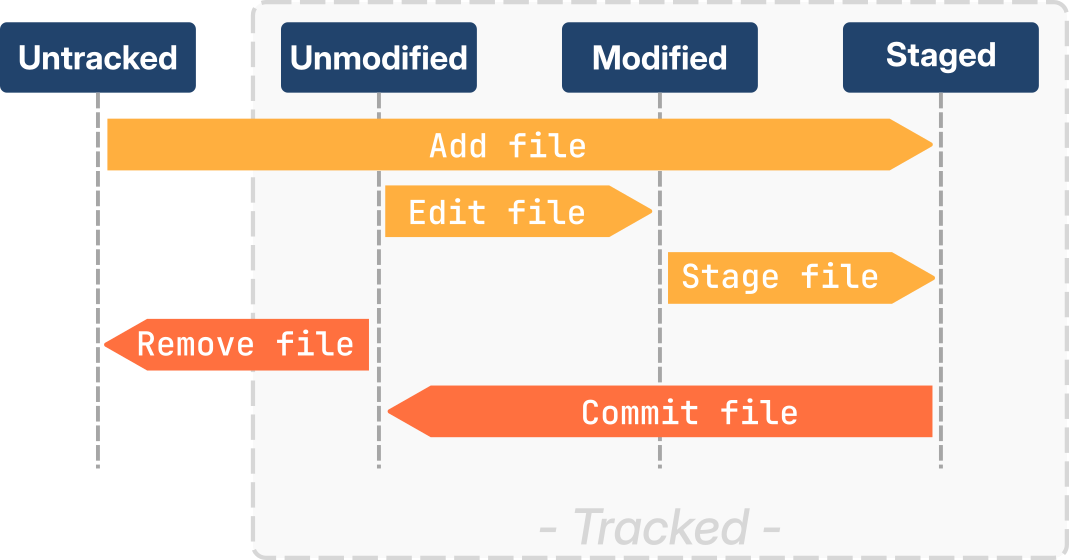
\includegraphics[scale=1]{Images/workingTree_tracked.png}
    \caption{illustrates how files move through the different tracking categories.}
\end{figure}

\subsection{Lifecycle States of Tracked Files}
GGit records your work through several \textit{storage stages}, each representing a deeper level of permanence:
\begin{enumerate}
     \item \textbf{Stashed} --- work in progress is temporarily stored aside, allowing you to return to a clean working state.
    \item \textbf{Modified} --- a tracked file has been changed in your \textbf{working directory} but not yet staged.
    \item \textbf{Staged} --- you have marked a modified file in its current version to go into your next \textit{commit snapshot}.
    \item \textbf{Committed} ---  the snapshot has been saved to your \textbf{local repository}.
    \item \textbf{Pushed} --- the commit has been transferred to a \textbf{remote repository}.
\end{enumerate}

\begin{figure}[H]
\centering
    \centering
    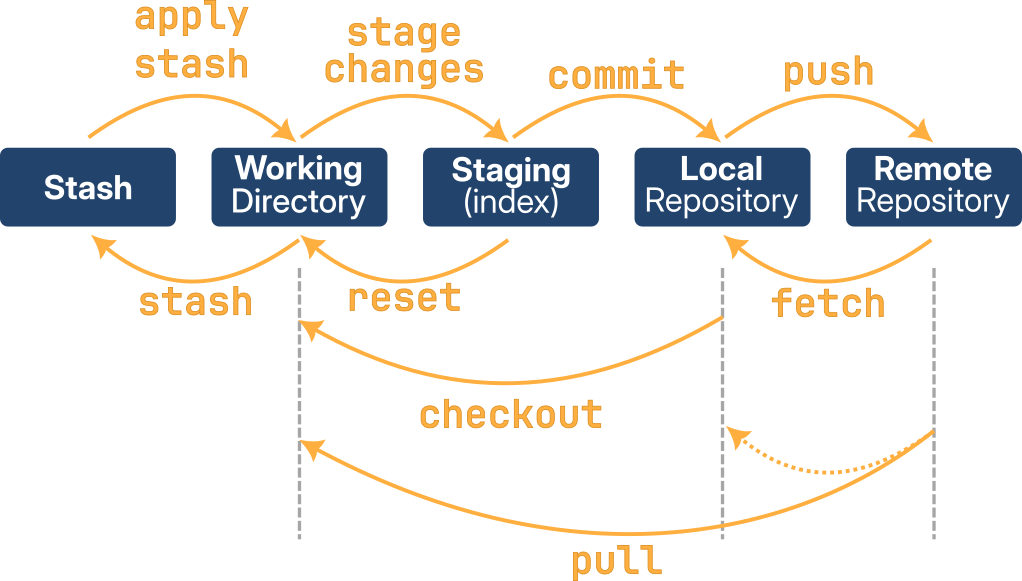
\includegraphics[scale=1]{Images/recordingChanges.png}
    \caption{illustrates how files move through these stages during normal Git operations.}
\end{figure}
    
\section{Commit Lifecycle}
The commit lifecycle begins by checking the state of files, then adding the desired files to the staging area, and finally committing them to the repository. Commits can also be pushed to a remote repository.

\subsection{File States}
To check the states of our files we can use:
\begin{gitBashBox}
status
\end{gitBashBox}
\noindent Adding the \textit{short} flag\footnotemark[2] gives a more concise output, if the regular one is too long. The \gitinline{status -s} and \gitinline{tsatus --short} syntax are synonymous to one another.
\begin{table}[H]
    \centering
    \begin{tabular}{c|l}
       \hspace{2mm} M  & modified but not staged\\[2pt]
       M\hspace{3mm}   & modified and staged\\[2pt]
       MM  & modified, staged and then modified again \\[2pt]
       A\hspace{3mm}   & new files added to staging area \\[2pt]
       ?\hspace{0.7mm}?  & new files that aren't tracked \\
       
    \end{tabular}
    \caption{Shorthand symbol meaning}
    \label{tab:short_symbols}
\end{table}

\noindent If \textit{git status} is too vague, use \gitinline{git diff} it shows changes between your working directory and the staging area. \textbf{→ unstaged changes}\newline
\gitinline{git diff --staged} and \gitinline{git diff --cached}\hspace{1mm}\footnotemark[3]\hspace{0.2mm} will shows changes between the staging area and the last commit.  \textbf{→ staged changes}

If you have a newly untracked directory with a bunch of untracked files \gitinline{git diff} will only show you the untracked directory, not all the files inside that aren't tracked either. To see these you can \gitinline{dit diff -uall}, which is short for \gitinline{git diff --untracked-files=all}.
\subsection{Tracking and Staging}
\noindent Track and stage new files using:
\begin{gitBashBox}
add <file>
\end{gitBashBox}
\noindent The git add command takes a path name for either a file or a directory; if it’s a directory, the command adds all the files in that directory recursively.

\subsection{Committing staged changes}
When the staging area is set up the way you want it, you can commit your changes with \gitinline{git commit}. This will however open a text editor for you to enter your commit message and if using the \gitinline{-v} verbose tag, will display more information on what will be commited.\newline
Becasue we are lazy we can use:
\begin{gitBashBox}
commit -m "message"
\end{gitBashBox}
This allows us to skip the editor step and type up our comment in the editor itself.\newline

If you want to skip the staging are, one can add the \gitinline{-a} flag. This will  also add all tracked files.

\subsection{Pushing to Remote}
If you are working with a remote repository, you will want to push your changes to it using \gitinline{git push}.

\section{Mistaken commit}
If you have made a mistake or forgot something either undo the changes or amend the commit.
\begin{enumerate}
    \item \gitinline{git add} any files you forgot, and then:
    \begin{gitBashBox}
    commit --amend -m "your message"
    \end{gitBashBox}
    This will amend your commit. If you have already pushed you will need to \gitinline{git push --force-with-lease}. \textcolor{red}{\bfseries Caution:} This rewrites commit history, because the amended commit gets a new hash! If others have already pulled the old commit, they’ll need to sync manually.
\item This will simply reset your commit to right before you made it:\footnotemark[4]
    \begin{enumerate}
    \item Undo last commit but keep changes staged
    \begin{gitBashBox}
reset --soft HEAD~1
    \end{gitBashBox}
    \item Undo last commit and unstage changes
    \begin{gitBashBox}
reset --mixed HEAD~1
    \end{gitBashBox}
    \item Undo last commit and discard changes
    \begin{gitBashBox}
reset --hard HEAD~1
    \end{gitBashBox}
\end{enumerate}
\end{enumerate}



\subsection{Undo when pushed}
\begin{gitBashBox}
revert <commit>
\end{gitBashBox}
Where <commit> is the commit hash.
Use \gitinline{git log} or \gitinline{git log --oneline}.
\gitinline{git --no-pager log} doesn't leave you in the pager, which you would normally equit with \textbf{q}.


% --- Footnotes ---
\footnotetext[1]{A Snapshot is your last commit, see Glossary for more details.}
\footnotetext[2]{A flag is a parameter you pass to a Git command to modify its behavior. There are short (-s) and long (-\hspace{0.1mm}-short) flags. Functionally \textit{most} Git commands treats them the same.}
\footnotetext[3]{-\hspace{0.1mm}-chaced is older terminology}
\footnotetext[4]{HEAD points to your current commit (the one your working directory is based on)}